\section{Methoden} \label{sec:Methoden}
			
	\begin{figure}[ht]
		\centering
		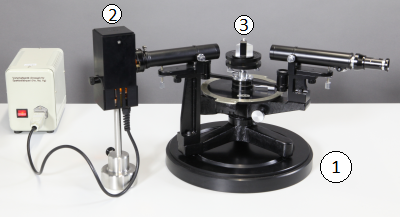
\includegraphics[width=0.7\textwidth]{bilder/aufbau.png}
		\caption{Darstellung des Versuchsaufbau. Dabei ist (1) das Spektrometer, (2) die Lichtquelle und (3) ein Prisma.\cite{WWU}}
		\label{fig:aufbau}	
	\end{figure}	
	Der grundlegende Aufbau ist in Abb. \ref{fig:aufbau} dargestellt und für alle Teilversuche gleich.
	Dabei ist (1) das Spektrometer, (2) die Lichtquelle und (3) ein Prisma.
	Die Lichtquelle soll so auf das Spektrometer gerichtet werden, dass das Licht durch eine Spaltblende an dem einem Arm des Spektrometers verläuft und auf das Prisma trifft.
	An dem anderem Arm befindet sich ein Okular mit einem Fadenkreuz, sodass die erkennbaren Spektrallinien eingeordnet werden können.
	Dazu dient eine Gradskala auf dem Spektrometer.
	An dieser lässt sich der Winkel ablesen bei dem das Fadenkreuz in dem Okular liegt.
	
	Als erstes soll eine Natriumdampflampe als Lichtquelle verwendet werden und das Prisma so in den Strahlengang gebracht werden, dass dieser symmetrisch durch das Prisma geht.
	Darauf soll das Linienspektrum von Natrium hinter dem Okular betrachtet und die Beobachtungen erläutert werden.
	Anschließend soll mit einem 300-Spalt-pro-\si{\milli\meter} Transmissionsgitter statt des Prismas das Linienspektrum betrachtet werden.
	Analog dazu danach mit einem Gitter mit doppelt so vielen Spalte pro \si{\milli\meter}.
	Für die drei verschiedenen dispergierenden Elemente soll das Auflösungsvermögen anhand der Beugungsordnungen und der Na $D$-Linie diskutiert werden.
	
	Bei dem zweitem Teilversuch soll zur Bestimmung des Gases in einer Energiesparlampe zunächst das Linienspektrum einer Heliumlampe herangezogen werden.
	Hier soll weiterhin das 600-Spalt-pro-\si{\milli\meter} Transmissionsgitter verwendet werden.
	Eine Tabelle der Wellenlängen die den einzelnen Spektrallinien zugehören ist für diesen Versuch gegeben.
	Mit Hilfe der Tabelle, des Fadenkreuzes an dem Okular und der Gradskala soll eine Funktion für die Wellenlänge in Abhängigkeit des Winkels durch diese Spektrallinien erstellt werden.
	Daraufhin soll das Linienspektrum der Energiesparlampe betrachtet werden und anhand der Wellenlängen, die sich aus der aufgestellten Funktion ergeben, das Gas identifiziert werden mit dem die Lampe gefüllt ist.
	
	Für den letzten Teilversuch sollen die Spektren verschiedenfarbiger Leuchtdioden betrachtet werden.
	Dazu sollen die Wellenlänge des Emissionsmaximum bestimmt werden.
	Auch hier soll die Beobachtung mit dem 600-Spalt-pro-\si{\milli\meter} Transmissionsgitter durchgeführt werden.
	Zudem soll für jede der Dioden die Spannung gemessen werden, ab der sie zu leuchten beginnen.
	Zuletzt sollen die zugehörigen Spannungen als Funktionswerte des Kehrwerts der entsprechenden Wellenlänge aufgetragen werden und $hc$ daraus bestimmt werden.
	
\section{Durchführung}
		
	Da andere Gruppen den Versuch bereits zuvor an dem selben Spektrometer durchgeführt hatten, war die Justierung des Spektrometers bereits erledigt, wurde jedoch vor Beginn der Messung überprüft.
	
	Die Durchführung erfolgte analog zu der Beschreibung in Abschnitt \ref{sec:Methoden}.
	Hierbei traten keine unerwarteten Effekte auf.
	
	Für die Natriumdampflampe ließ sich nur eine breite gelbe Spektrallinie und einige weitere schwächere beobachten (darunter eine blaue, eine türkisfarbene, eine grüne und eine rote).
	Bei den Gittern hingegen ließen sich ab den zweiten Beugungsmaxima jedoch schon zwei gelbe Linien, welche sehr nah aneinander lagen erkennen.
	Der Abstand zwischen diesen wurde mit höheren Beugungsmaxima größer.
	Mehr als vier Maxima pro Seite ließen sich jedoch nicht beobachten.
	
	Die Winkel der beiden gelben Natriumlinien, sowie der für das Helium- und Energiesparlampenlinienspektrum sind dem Laborbuch zu entnehmen.
	
	Bei den Leuchtdioden wurden jeweils eine rote, gelbe, grüne und blaue verwendet.
	Das nullte Maximum entsprach bei allen Dioden einer Linie in ihrer Farbe.
	Die ersten Maxima jedoch waren für alle Dioden wie verschmierte Bänder und einzelne Maxima waren nur schwer zu erkennen.
	Alle Bänder besaßen einen Farbverlauf, welcher einen Teil des Gesamtspektrums ausmachte.
	Bei der roten Leuchtdiode war das Band nahezu komplett rötlich, das der gelben jedoch hatte bereits eine kontinuirliche Verteilung von grün bis rot.
	Für die grüne Leuchtdioden traten die Farben von türkis bis rot auf und bei der blauen alle von violett bis rot.
	Die Intensität war jedoch bei letzteren drei bei ihrer eigenen Farbe (gelb, grün bzw. blau) am höchsten.
	Vor Betrachtung der Linienspektren wurde für jede der Dioden die Einsatzspannung drei mal gemessen, da die Unsicherheit für eine einzelne Messung zu groß wäre.
	Bei diesen fällt auf, dass die Einsatzspannungen der Dioden mit Anteilen geringerer Wellenlängen höher liegen als andere.   
		
\section{Datenanalyse} \label{sec:Analyse}
	
	%TODO Natrium
	
	Nun zu dem Linienspektrum des Heliums.
	Da nicht alle Spektrallinien aus der Tabelle den beobachteten zuzuordnen waren wurden, wurden nicht alle zu der Aufstellung einer Funktion der Wellenlänge verwendet.
	\begin{figure}[ht]
		\centering
		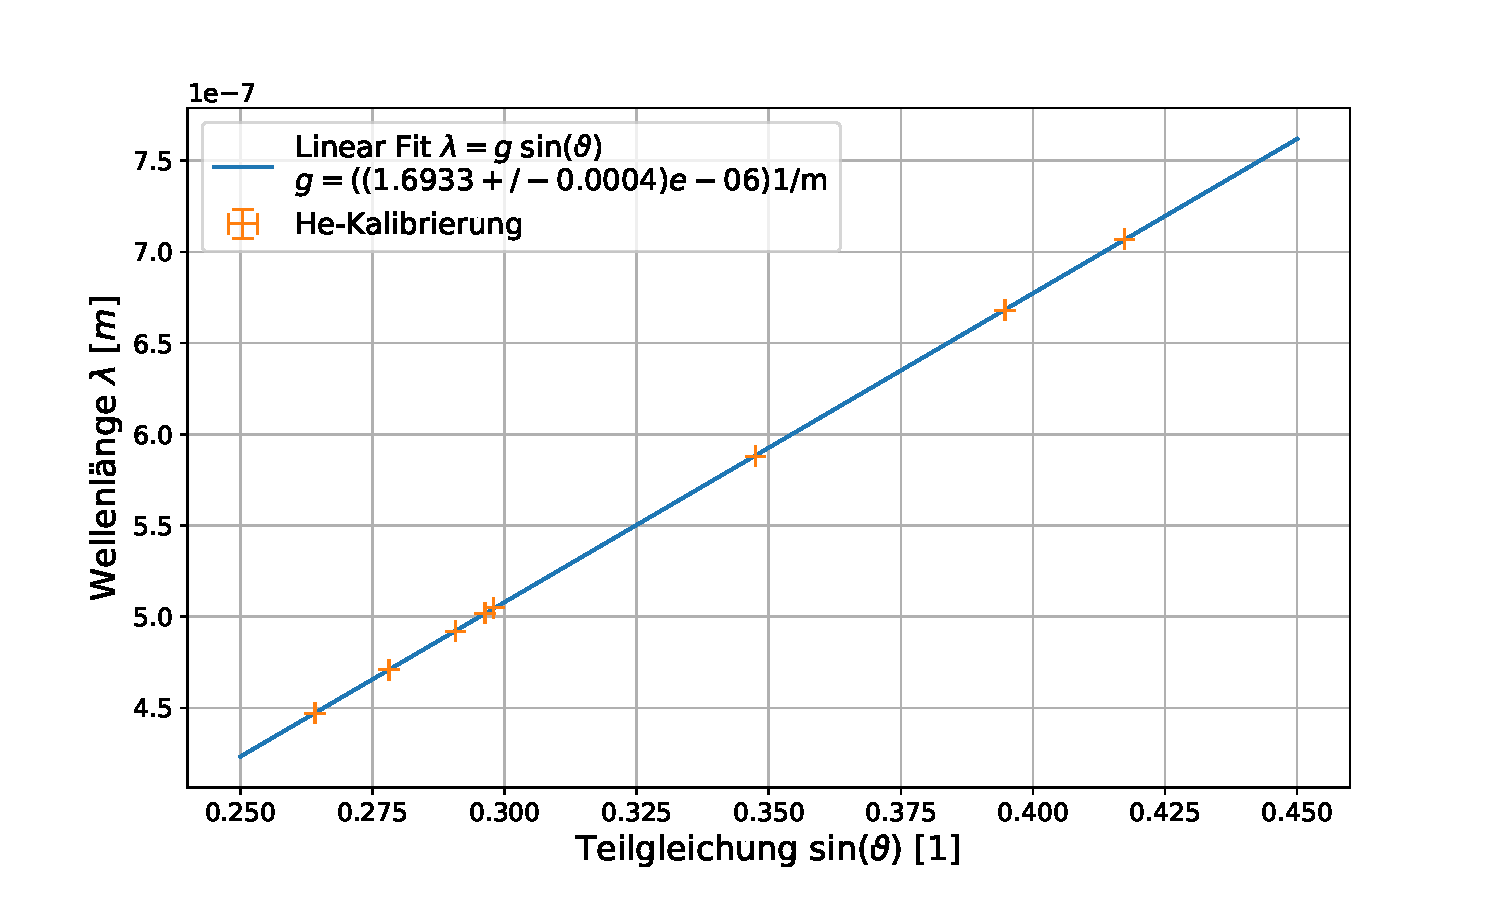
\includegraphics[width=\textwidth]{data/GitterConstPruef.pdf}
		\caption{Darstellung der Wellenlänge in Abhängigkeit des Sinus des gemessenen Winkels für die Heliumlampe mit linearerem Fit.}
		\label{fig:Funktion}	
	\end{figure}
	Abbildung \ref{fig:Funktion} stellt den Zusammenhang zwischen den gemessenen Winkeln der Spektrallinien und dazu zugehörigen Wellenlängen dar.
	Damit ein linearer Fit verwendet werden konnte wurde der Sinus der Winkel aufgetragen.
	Das lineare Verhältnis folgt aus:
	\begin{equation}
		\Delta\lambda = \Delta\sin{\vartheta_m} \frac{g}{m},
	\end{equation}
	wobei $m$ die Zahl des Beugungsmaximums	und $g$ die Gitterkonstante ist.
	\begin{figure}[ht]
		\centering
		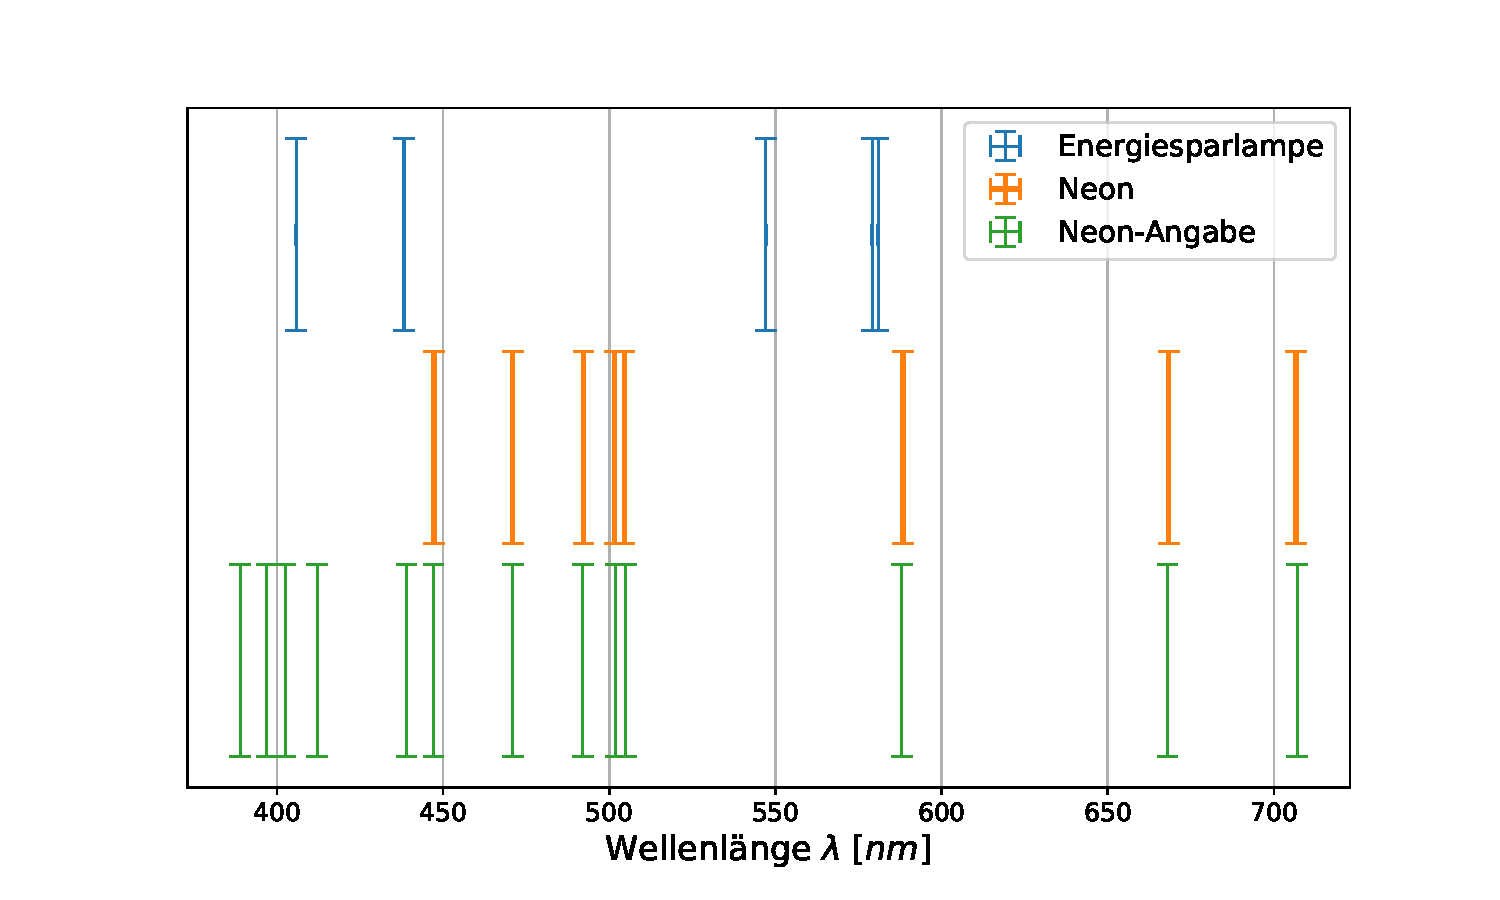
\includegraphics[width=\textwidth]{data/EnergieSpar.pdf}
		\caption{Darstellung der Spektrallinien der Werte für Helium aus der Tabelle (grün), der gemessenen für Helium (orange) und der gemessenen der Energiesparlampe (blau).}
		\label{fig:Linien}	
	\end{figure}
	Hiermit und mit den Winkeln für die Energiesparlampe ergaben sich die Ergebnisse in Abb. \ref{fig:Linien}.
	Die fünf erkennbaren Linien für die Lampe liegen bei \SI{}{\nano\meter}, \SI{}{\nano\meter}, \SI{}{\nano\meter}, \SI{}{\nano\meter} und \SI{}{\nano\meter}.
	
	\begin{figure}[ht]
		\centering
		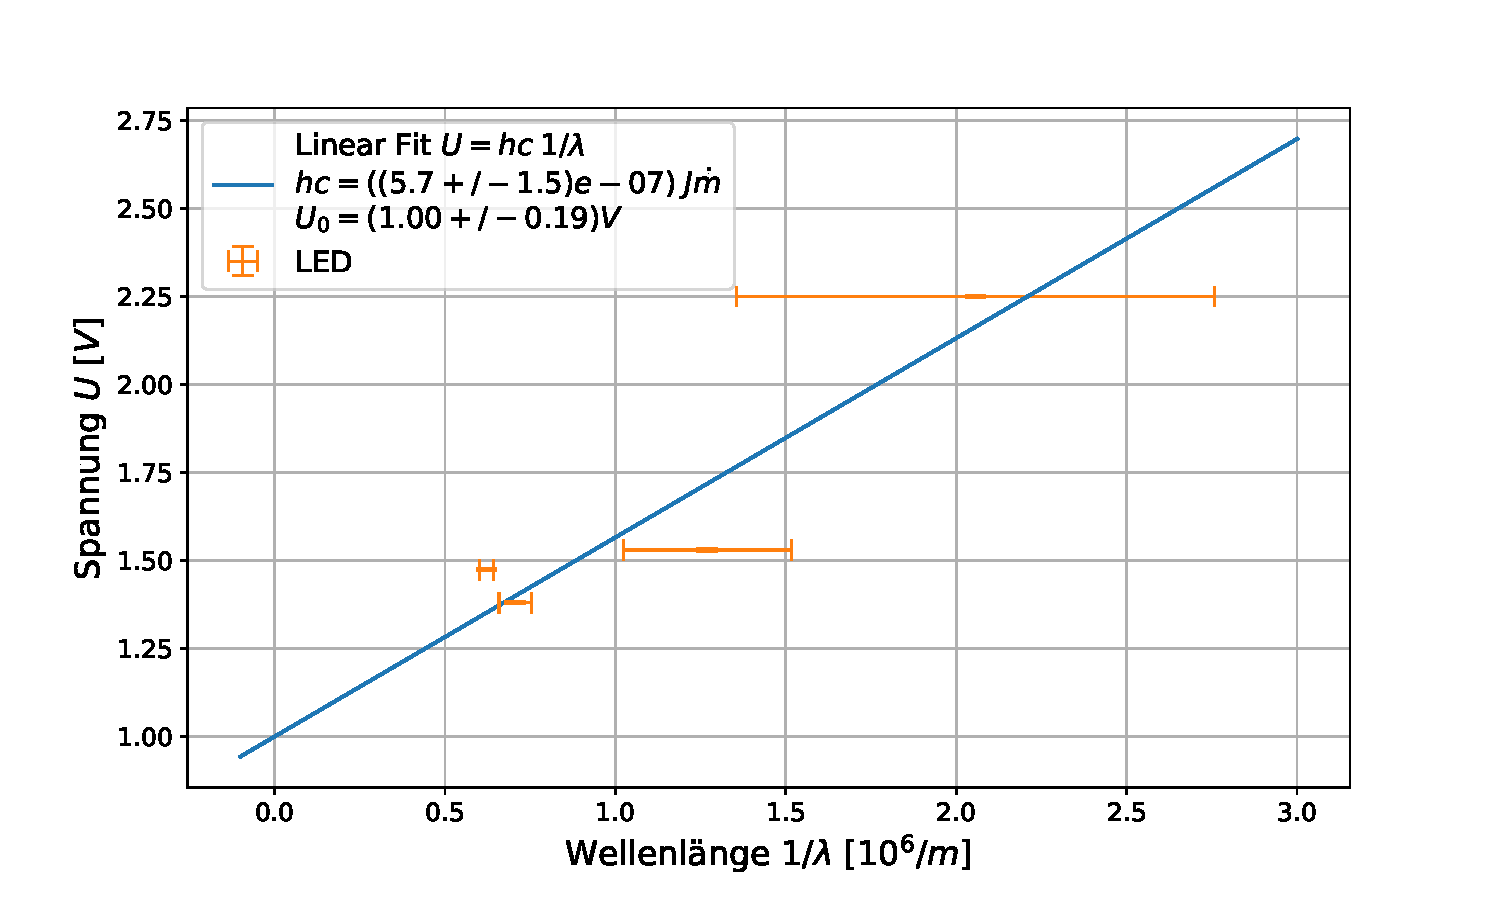
\includegraphics[width=\textwidth]{data/Dioden.pdf}
		\caption{Darstellung der Einsatzspannung für die vier verschiedenen Wellenlängen, bei denen die Intensitätsmaxima der einzelnen Dioden liegen. Zudem linearer Fit um $hc$ zu bestimmen.}
		\label{fig:Dioden}	
	\end{figure}
	Bei dem letzten Teilversuch mit den Dioden ergab sich durch auftragen der gemittelten Spannungswerte der in Abb. \ref{label} dargestellte Verhalt. 
	Dabei sind die Messpunkte %TODO Dioden
			
\section{Diskussion}
